\documentclass{article}
\usepackage{graphicx} % Required for inserting images
\usepackage{placeins}

\title{Kirby}
\author{Ximena Guadalupe Vidals Muñoz}
\date{25 de septiembre de 2026}

\begin{document}

\maketitle

\section{Introducción}
Kirby es de mis videojuegos favoritos, lo conocí gracias a Super Smash Bros, antes de hacer esta tarea no sabía que kirby tenía tantos juegos y tanto lore, yo solo he jugado Kirby and the Forgotten Land el cual ya acabé y es el primer juego de kirby que jugue, después me regalaron Kirby's Return to Dream Land y ese no lo he acabado pero ya me se el lore de ambos. \\
Como mencioné en un inicio, solo me centraré en el lore de estos dos juegos porque son los que conozco y al final mencionaré todos los juegos que se que tiene kirby. 

\section{Kirby's Return to Dream Land }
En una cronología, Kirby's Return to Dream Land va antes que Kirby and the Forgotten Land, así que iniciaré con el lore de este, quisiera aclarar que esta es la forma en que entendí la historia y tal vez algunas cosas sean más interpretación mia que el lore real. \\ 
\\
Todo inicia con una Kirby y sus amigos existiendo muy felices y teniendo una vida tranquila hasta que una nave con forma de barco se estrelló contra Dream Land y fue perdiendo poco a poco sus piezas por todo el planeta, en este barco nave venía Maglor el cual les pide a Kirby y sus amigos recolectar las piezas faltantes de su nave y como agradecimiento los llevaría a el lugar de donde el provenía. \\ \\
Después de lograr recolectar todas las piezas de la nave de Maglor, los lleva a el lugar de donde provenía y se encuentran a un dragón llamado Landia, este dragón es de 4 cabezas  y tenía una corona. \\ \\
Después de una batalla entre Kirby y sus amigos contra Landia, los amigos de Kirby ganan y Landia suelta la corona, Maglor toma la corona y dice que engañó a Kirby y a sus amigos, una vez que Maglor se pone la corona, se transforma y revela que la corona es para dominar todo el universo y que iniciaría con el Planeta de Kirby \textit{Pop Star}. \\ \\
Landia se une con Kirby y sus amigos para derrotar a Maglor y salvar a todo el universo, como Kirby es increíble, logran derrotar a Maglor y luego al alma de Maglor unida con la corona. \\ \\
Después de todas estas batallas, Kirby y sus amigos pueden regresar a Dream Land a continuar sus vidas, la siguiente parte del juego es Maglor luchando con su poder esparcido por distintas dimensiones y así poder recuperar su poder. \\ 
Al final Maglor logra vencer a la parte malvada de él que lo controlaba y salió de esa dimensión para iniciar una nueva vida como un mago bueno y renovado. :D 

\begin{figure} [h]
    \centering
    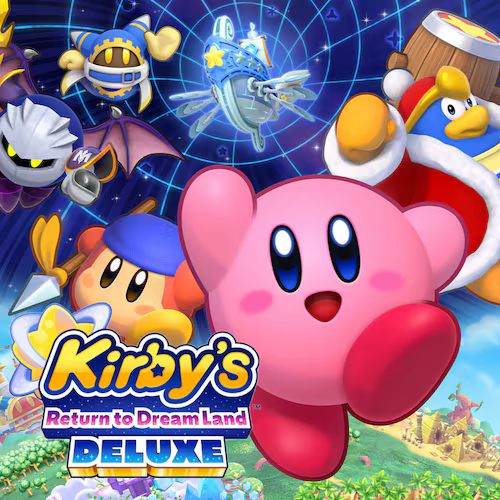
\includegraphics[width=0.5\linewidth]{imagen.png}
    \caption{Kirby's Return to Dream Land Deluxe}
    \label{fig:placeholder}
\end{figure}

\section{Kirby and the Forgotten Land}
Este juego tiene una historia creo que un poco más larga, así que me saltaré algunos detalles y lo resumiré lo más que pueda. \\ \\
Este juego inicia con Kirby viviendo tranquilamente en Pop Star y paseando en su estrella hasta que se abre una grieta en el cielo que comenzó a absorber todo incluyendo a Kirby y a los Waddle Dees, luego de viajar en el portal, Kirby aparece en una ciudad abandonada y explorando llega a un centro comercial, en este centro comercial absorbe un auto y se pone a pasear por toda la ciudad. \\ \\
Después de Kirby paseando, se da cuenta que los Waddle Dees estan siendo secuestrados y conoce a Elfilin que fue salvado por Kirby, se hacen amigos y juntos deciden ir a salvar a todos los Waddle Dees que estaban siendo secuestrados. \\ \\
Kirby se enfrenta a muchos villanos de distintos lugares, los cuales si no recuerdo mal fueron una pradera, una playa, un circo, un lugar con hielo, en este último lugar el rey Dee Dee malvado secuestra a Elfilin. \\ \\
Para rescatar a Elfilin, Kirby tiene que viajar a la nación prohibida, aquí tiene una batalla con Armadiloco y después con una versión aun más malvada de el Rey Dee Dee, derrota a ambos y tras derrotar al Rey Dee Dee lo hace entrar en razón y se hace bueno de nuevo. \\ \\
Cuando el Rey Dee Dee entra en razón, se abre una puerta detrás de ellos, solo logra entrar Kirby y un Waddle Dee, esta puerta es un ascensor donde escuchan un mensaje de bienvenida que les cuenta como están en un laboratorio y en este laboratorio se encuentra un alienígena y Elfilin secuestrado. \\ \\
Elfilin es la otra mitad del alienígena y lo secuestran porque gracias a él, los habitantes de la tierra olvidada podrán teletransportarse para ir a un nuevo mundo, Kirby logra derrotar a Leongar y así salvando a Elfilin. \\ \\
El alienígena despierta y absorbe a muchas bestias haciéndose más fuerte, Kirby y Elfilin tratan de escapar pero el alienígena absorbe a Elfilin, se transforman en una esfera y se van volando. \\ \\
Kirby ve como Elfilin y el alienígena se transforman en Fecto Elfilis que desafia a Kirby sobre un edificio, Kirby después de una batalla muy épica logra salvar a Elfilin pero Fecto Elfilis abre un portal para estrellar Pop Star en la tierra olvidada, Kirby se transforma en un camión para ir contra Fecto Elfilin y después de otra épica batalla logran vencerlo. \\ \\
Pero Pop Star ya estaba siendo destruido y absorbido por el portal, Elfilin se va al portal para poder cerrarlo y se sacrifica para lograrlo o eso creímos todos, Elfilin aparece detrás de Kirby y le explica que lo ayudó Zarparina, ella igual los demás jefes que antes eran malvados ahora son aliados de Kirby. \\ \\
Se abré otro portal donde comienzan a buscar a Leongar porque Zarparina les pidió ayuda, después de otras batallas más en los planetas de ese portal, llegan con Leongar y tratan de salvarlo con sus recuerdos pero como Kirby es buenísimo logran salvarlo, llegan varios personajes con los fragmentos del alma de Leongar y despierta. \\ 
Finalizando el juego con Kirby y todos sus nuevos amigos siendo felices en Dream Land. 

\begin{figure}[h]
    \centering
    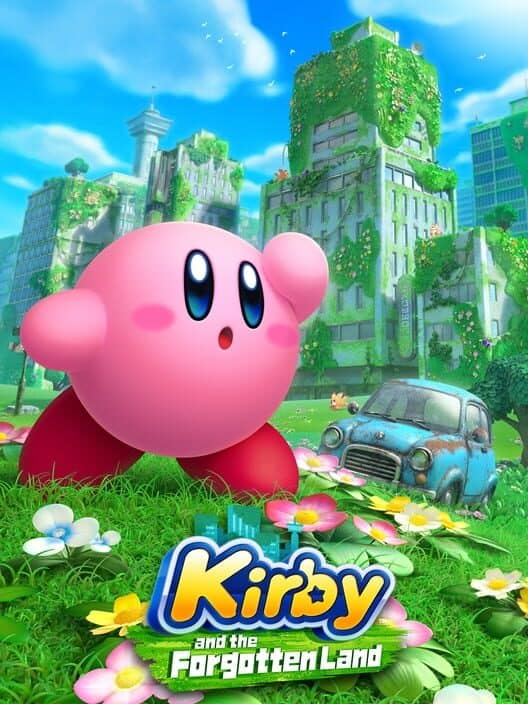
\includegraphics[width=0.5\linewidth]{imagen2.png}
    \caption{Kirby and the Forgotten Land}
    \label{fig:placeholder}
\end{figure}
\FloatBarrier %

\section{Juegos de Kirby}
\begin{itemize}
    \item Kirby's Dream Land
    \item Kirby Nightmare in Dream Land
    \item Kirby Super Star
    \item Kirby's Dream Land 2
    \item Kirby's Dream Land 3
    \item Kirby 64: The Crystal Shards
    \item Kirby and the Amazing Mirror
    \item Kirby Canvas Curse
    \item Kirby Squeak Squad
    \item Kirby Mass Attack
    \item \textbf{Kirby's Return to Dream Land Deluxe}
    \item Kirby's Epic Yarn
    \item Kirby and the Rainbow Curse
    \item Kirby Triple Deluxe
    \item Kirby Planet Robobot
    \item Kirby Star Allies
    \item \textbf{Kirby and the Forgotten Land}
\end{itemize}
\section{Final}
Después de este increíble relato sobre el lore de solo 2 juegos de Kirby, puedo concluir que Kirby tiene demasiado lore y tendrá más con el próximo juego. \\
Quisiera decir que Kirby me inspirá a ser mejor persona y que \textit{Kirby le gana a todos}, gracias por esta tarea donde pude saber más sobre mi personaje favorito y Kirby es maravilloso y merece todo su reconocimiento aunque debería ser más famosa la historia de todos los juegos. 
\end{document}
